\documentclass[english]{tktltiki}
\usepackage[pdftex]{graphicx}
\usepackage{subfigure}
\usepackage{url}
\usepackage{algpseudocode}
\usepackage{algorithm}
\usepackage{amssymb}
\usepackage{amsmath}
\usepackage{graphicx}


\DeclareMathOperator*{\argmax}{arg\,max}
\begin{document}
%\doublespacing
%\singlespacing
\onehalfspacing

\title{Big Data Influence Maximization blah balh}
\author{Behrouz Derakhshan}
\date{\today}

\maketitle

\numberofpagesinformation{\numberofpages\ pages + \numberofappendixpages\ appendices}
\classification{\protect{\ \\
A.1 [Introductory and Survey],\\
I.7.m [Document and text processing]}}

\keywords{layout, summary, list of references}

\begin{abstract}

Network influence maximization. Something about graphs, about network influcence, social network, other related areas, big data, hadoop and other technologies, graph processing

\end{abstract}

\mytableofcontents

\section{Introduction}
The term graph, first used by mathematician J. J. Sylvester, is a representation of set of objects, some of which are connected. Typically, in a graph the interconnected components are called \textbf{vertices}, and the links that are connecting them are called edges. Graph theory, is the field of mathematics that studies graphs and since its introduction, it has been used extensively, in many branches of science. In computer science, graphs can represents, networks of computers and the communication between them, it can represent websites and the links between them. In Chemistry and Physics, graphs are used to model the atoms and molecules and their interactions. In sociology, relation between actors, directors and movies can be depicted using a graph. And most notably is the its use case in social networks and modeling the relationship between people (friendship, acquaintance) . \\
Graphs components, can carry extra information, for example the edges can carry weight which can quantify or qualify the connection between two nodes. For example in a graph that represent geographical locations, where vertices (nodes) represent places, the edges represent the length between the locations. \\
With introduction of online social networks, an enormous amount of information is now available . One application that has been studied in social network or in graphs in general is the spread of information between nodes, based on the structure of the graph and the edge weights. In medicine and biology it has been used to find the spread of a disease either to find the initial person who contracted the disease or finding key vertices that could amplify the spread and by identifying those nodes further spread of the disease can be avoided. It has use cases in marketing as well, in which the aim is to find key people in a social network, that can spread the information among their friends and acquaintances, and for example by offering discount to a certain group of people they can rely on the work-of-mouth phenomena. \cite{kempe03} has defined models in which network propagation can be studied, and how to maximizes the the propagation in a network. \cite{domingo01} studied how to find the value of a customer in a network and how to use that to influence other customers. Influence maximization that is the topic of this thesis, has been studied for more than a decade now, but with the massive amount of available data, the scalability has become an issue. Some websites, such as Facebook, Twitter, Amazon, ... carry Terabytes and in some cases Petabytes of data related to their customers and their relationship. And the models developed for simulating the network propagation and finding the initial set that maximizes the influence, they will all suffer greatly when applied to graphs of this magnitude. \\
Over the past couple of years, many platforms for processing huge amount of data has been developed. This branch of computer science, named BigData, has gain a lot of attention lately. Some of the most notable frameworks are Hadoop and Spark. Hadoop is open source project that is based on Google's MapReduce framework. 
Using these and other similar frameworks, many graph processing tools and applications are built which utilizes the mechanism of these frameworks to process graphs of millions or billion of nodes and trillions of edges. \\
The most widely used frameworks for processing big graphs, are :
\begin{itemize}
\item 
Giraph which is open source project by on Google's Pregel framework. It is built on top of Hadoop
\item 
GraphX is open source project built on top of Spark
\item
Graphlab and open source project written in  and C++ . 
\end{itemize}
In this thesis, I will study the performance penalty of running state of the art algorithms for network propagation, more specifically the Independent Cascade method (which will be explained in the next section) . And propose and implement distributed methods for the algorithm written for GraphLab, GraphX and Giraph and comparison between each frameworks will be made. 
The rest of this document is organized as follow; in section 2, Big Data frameworks, graph frameworks, influence maximization methods are studies. In section 3, a distributed algorithm and implementation methods are presented. In section 4, comparison of the distributed and single node implementations as well as the difference between each graph framework are studied . In section 5 conclusion blah blah
In the next sections, different Big Data platforms are studied in details. Graph processing frameworks are explained extensively. And current and state of the art algorithms for network propagation and influence maximization are studied. 




\section{Literature Review}

\subsection{Big Data}
Information and data has always been gathered for analysis and improvement or invention of new or existing technologies. It had helped governments to better govern countries, it had helped companies to better understand their costumers, and it had helped researchers and scientists to solve problems. With introduction of World Wide Web(http://webfoundation.org/about/vision/history-of-the-web/) exchange and collection of data has become a lot simpler. Big firms and companies started to collect user's information, browsing behavior and etc . Petabytes of data are being stored and exchanged everyday, and these data contain valuable information that is being used for solving a lot of problems using data mining and machine learning methods. 
Processing this amount of data, has never been an easy tasks and prior to introduction of new BigData technologies, this processing and analyzing has been always done using expensive Server systems that are able to process millions to billions of bytes of data in a second. 
Google Inc. revolutionary papers has drastically changed field. \cite{ghemawat03} introduced \textbf{The Google's Distributed System}; a file system built for storing terabytes of data. It is scalable, meaning more storage can be easily added, and it is being deployed on commodity hardware, meaning it does not require any sophisticated and expensive piece of hardware to use. Dean et. al \cite{dean04} introduced \textbf{MapReduce} a framework for processing large amount of data, again it is scalable and it can be deployed on commodity hardware. 
Although the source code either of these two technologies were never released by Google, but based the publications \textbf{Doug Cutting} created the open source project \textit{Hadoop} which implements both MapReduce (Hadoop's MapReduce) and Google File System (Hadoop Distributed File System or HDFS for short). Since then, Hadoop has become BigData standard, several new technologies and project have been added to it.

\subsubsection{Hadoop}
Hadoop is consists of two major parts. 
\textbf{MapReduce} which is a parallel programming paradigm. It is designed to run on distributed systems with many commodity computers. It involves three main steps, namely \textit{Map}, \textit{Reduce} and \textit{Shuffle}. The first two are defined by the user. Map operations are run in parallel and they process the data individually, data is divided into different portions and each one is processed by a mapper. The result of the mappers are send to a Reduce task(or several) where the results are combined. A shuffle operation is usually performed on the result of the Map so that similar data are all send to the same nodes. Below is a simple algorithm for counting words in a series of documents. 

\begin{algorithm}
\begin{algorithmic}
\Function{map}{String name, String document}
\State {//name: document name}
\State{//document: document contents}
   \For {each word w in document}
      		\State emit (w, 1)
   \EndFor
\EndFunction
\State 
\Function {reduce}{String word, Iterator partialCounts}
\State{//word: a word}
\State{//partialCounts: a list of aggregated partial counts}
  \State sum = 0
  \For{ each pc in partialCounts}
    \State sum += ParseInt(pc)
    \State emit (word, sum)
\EndFor
\EndFunction
\end{algorithmic}
\end{algorithm}

\begin{figure}[ht!]
\centering
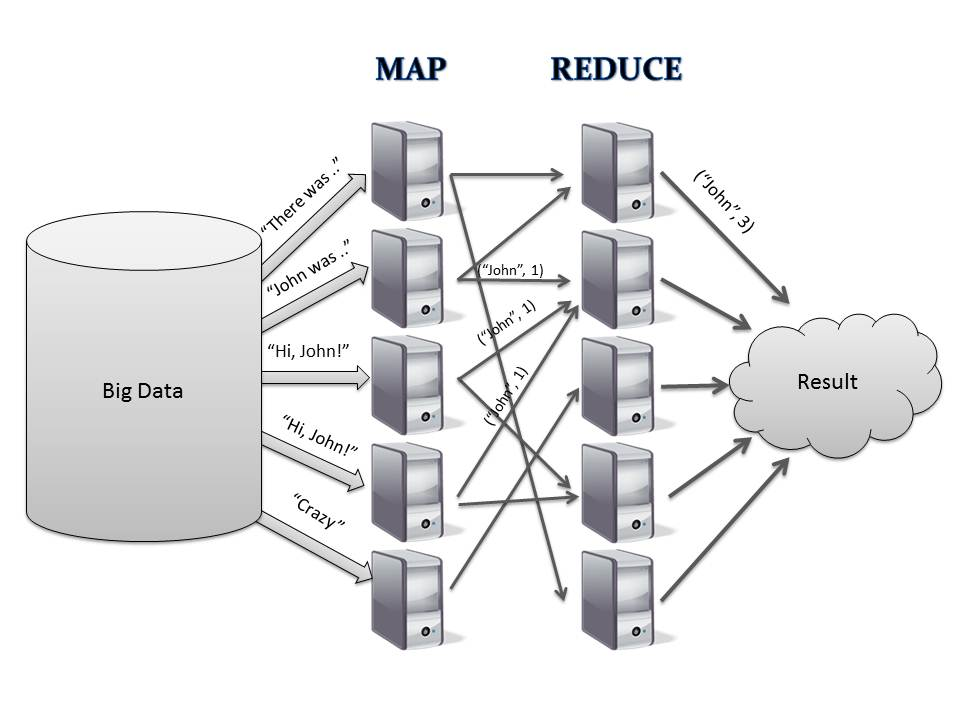
\includegraphics[width=130mm]{figures/mapreduce.jpg}
\caption{MapReduce paradigm}
\end{figure}

\textbf{Hadoop Distributed File System (HDFS)}
HDFS is a distributed file system, designed to run on commodity hardware. It provides high throughput access to application data and it fault tolerant. Though initially designed for Hadoop's MapReduce framework, it has been used in many different application.
\begin{figure}[ht!]
\centering
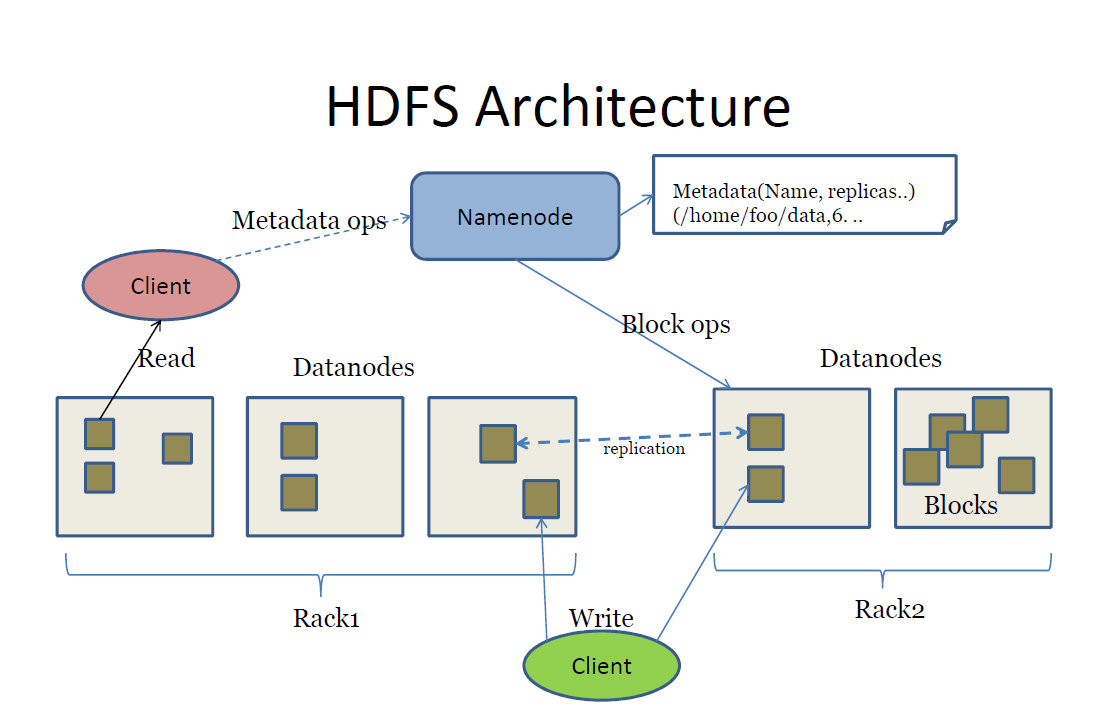
\includegraphics[width=130mm]{figures/hdfsarchitecture.png}
\caption{HDFS Architecture}
\end{figure}


\subsubsection{Spark}
What is Spark
\subsubsection{MPI}
What is MPI

\subsection{Graph}
Definition of Graph, a more detailed literate review. Maybe I can move some of the stuff from Introduction, or try to complement them

\subsubsection{Graph Frameworks}
Older graph frameworks, how they used work. A short overview of some important and common frameworks. Why there's a need for scalable frameworks

\subsubsection{Big Graph}
What is it, where does it come from, why is it important to have frameworks capable of processing massive graphs

\subsection{Giraph}
Apache Giraph is an iterative graph processing framework, built on top of Apache Hadoop. It is the open source version of Pregel by Google. 
\subsection{GraphX}
\subsection{Pregel}
Graph processing framework by Google. Pregel is a vertex centric computational model where each vertex process the incoming messages from the edges and pass along the output to the next vertices through edges. It is built for iterative processing and in a distributed environment. The API is similar to MapReduce where the users have to implement methods for two set of methods, the compute method and the aggregate method. Compute methods are executed on each vertex in parallel, there are mechansim involved however, to assert data consistency. The computations are done in steps called SuperStep. The main method is the compute method, where in each SuperStep a vertex will receive a list of messages from vertices in an arbitrary order, and after the processing is done, it will send messages to other vertices. The aggregator can collect global values from all vertices, they are usually  to keep track of some global counts or .... . 
\subsection{GraphLab}
GraphLab is a graph processing framework, tailored for big data sets. There are three versions of GraphLab :
\begin{itemize}
\item
Shared memory, multi-core parallel GraphLab
\item
Distributed GraphLab
\item
PowerGraph

\end{itemize} 


%\enlargethispage{5mm}
\subsection{Social Graphs}

\subsection{Influence Maximization}
Influence maximization problem is divided into two major parts. The first one is to find the graph of users (nodes) where edges between each user show the probability of  a user influencing the other. The second part is
based on this graph find a set of users that are proven to have the highest influence over others, in other words 
this limited group of users can maximize the influence through the network.

In \cite{kempe03} they have studied models by which influence propagates through social networks. They have discussed two diffusion models \\
\textit{Linear Threshold Model} and \textit{Independent Cascade Models} . In \textit{Linear Threshold Model} each node $v$ is influence by each neighbor $w$ acourding to a weight $b_v,w$ such that $\sum \nolimits_{w \, neighbor \, of \, v} b_v,w < 1$ . The diffusion process hence is as follows; each node $v$ will randomly chose a weight threshold $0 < \theta_v<1 $, this value determines tendency of node $v$ to become activated. Starting from the initial seed set, in each iteration for each node if the sum of the weight of its active neighbors become greater than the threshold then the node will become active, i.e. $\sum \nolimits_{w \, active neighbor \, of \, v} b_v,w  \geq \theta_v $. The process is deterministic however since $\theta_v$ is chosen at random, it shows our lack of knowledge their values. \textit{Independent Cascade Models} is a stochastic undeterministic process. It starts with an initial set of seeds, and in each time step $t$ every active node will try once to activate all of its neighbors, the probability of a node $v$ activating one of its neighbors $w$ is either define by a system property $p_v,w$ or is governed by the weight of the edge $w_v,w$. The process continues until no more new node can become active. 

The problem of influence maximization which is finding an initial set that will maximizes the profit( target function) is NP-hard . 
Formal definition : it asks for a parameter k, to find a k-nod set of maximum influence. They used approximation with a natural greedy hill-climbing strategy which will guarantee a 63 percent of the optimal solution performance (reference) . For the approximation to work , he target function should be sub-modular, they have proved that for both models the target function is indeed sub-modular.  They have run experiments on co-authorship in physics theory section of arXiv (www.arxiv.org) . The results show that their greedy algorithm performs better that other methods such as random selection, high-degree or central nodes discussed in book Social Network Analysis by S. Wasserman (find reference) \\
\cite{domingo01} discusses the use case of influence maximization in marketing. They first, described how to model a market as a social network. Making each individual user only dependent on its neighbors, the product and the marketing action(Markov random field). Through these a function was devised that calculates the global lift in profit given a marketing action was applied to some users. Starting from an initial configuration, using different optimization algorithms a local maxima for the function can be reached. 
They experimented on a collaborative filtering data set (MovieLenz) in which users have rated a list of movies. They have first constructed the network using the user rating, by choosing similar users( calculating the Pearson correlation coefficient of users) as neighbours . They have performed experiments on the data set and compared their method with mass marketing and direct marketing. Their method has increased the profit the most. Due to non-linearly of the model, it did not scale well for bigger size networks, hence they have proposed a new linear model \cite{domingo02}. Not only the new model decreased the computation time time, the simplified equation for calculating the network value of customers, made it easier to incorporate more complex marketing action. They have experimented with Epinions (cite) data set. Which is a website where users can rate items. It also has a feature called trusted users, where each user can select many other users as trusted sources of reviews. Domingo et .al, hence, applied their model to the dataset, but considering trusted users of a user his neighbors. Their experiments showed that a continuous marketing action (a marketing action that can have unlimited values, such as a discount) performs much better than boolean marketing actions (one that can either be true or false, such whether or not a discount should be given to a user with no regards for the amount of the discount ). 
\cite{cheng13} Have addressed both the accuracy and scalability of the solutions using the greedy methods. They have pointed out the main bottle neck in methods based on \cite{kempe03} are in the Monte Carlo simulation steps. They have proven that the objective function is not entirely sub-modular due to the randomness in the simulations, and hence to compensate for that many Monte Carlo simulations have to be run in each step of the algorithm which greatly reduces the performance. Present the proof here ....\\
They proposed a new method called StaticGreedy which uses precomputed a series of snapshots at the beginning of the algorithm and reuses those for every step of the greedy algorithm.  They have defined the two terms, snapshots and simulations which can be both used for the Monte Carlo simulations. \\
\begin{itemize}
\item 
Simulation : The influence spread is obtained by directly simulating the random process of diffusion triggered by a given seed set S.
\item
Snapshot : According to the characteristic of IC(Independent Cascade) model, whether u successfully activates v depends only on p(u,v). Hence prior to the main algorithm a Graph G$'$=(V,E$'$), which is a subgraph of G where an edge <u,v> is remained with the probability p(u,v) and deleted otherwise. 
\end{itemize}
Before the main steps of the algorithm plenty of snapshots are produced and averaged to estimate the spread function. 
Have StaticGreedy algorithm here :\\
1. Static snapshots \\
2. Greedy selection \\

Two main difference between this method and the previous ones are :
\begin{itemize}
\item
Monte Carlo simulations are conducted in static snapshot manner, which are sampled before the greedy process of selecting seed nodes
\item
The same set of snapshots are reused in every iteration to estimate the influence spread I(S), which explains the meaning of ''static''
\end{itemize}

They have performed experiment and compared their methods with the normal Greedy methods. None of the other greedy methods are any match with StaticGreedy in terms of speed and scalability. 

Saito and Kimura \cite{kimura06} have also investigated the scalability issue of ICM simulations. They have argued that the current simulation model in ICM requires many iterations and each iteration took a lot of processing time and power. They have proposed two natural special cases of the ICM such that a good estimate of this quantity can be efficiently computed. They define the Shortest-Path Model(SPM) which is a special case of the ICM such that each node v has the chance to become active only at step = d(A,v) , where if A is the initial set d(A,v) is the distance of A to node v. This means that each node is activated only through the shortest paths from the initial active set. The other model they have proposed named SP1M, which is each node v has the chance to become active only at steps t = d(A,v) and t =d(A,v) + 1. Through these two models they have proposed methods for calculating the spread of an initial set A. They have proved that the result achieved using this method is also within a bound of the best solution. In their experiments, they have assigned a uniform probably to each edge with two different values p = 0.1 and p =0.01. The experiments showed that the estimation of the spread for ICM increases as p increases while the processing times for the SPM and SP1M hardly change. They have also \\



\subsection{Learning Influence Probabilities}
\cite{goyal10} have tackled the problem of forming the social graph whose edges have the probability of a user
influencing the other based on a log of actions. Based on the General Threshold model that simultaneously 
generalizes the Linear Threshold and Independent Cascade models. They have formulated the problem like this :
given graph G = (V,E,T) with T being the time when each edge in the graph was constructed, an action log which contains relations Actions(User,Action, Time) which contains tuples indicating a user performed an action at certain time. The aim is to a function p : E --> [0,1] x [0,1] assigning both directions of each edge (u,v) in E the probabilities : $p_{v,u}$ and $p_{u,v}$.
Three different solution models were proposed. Static Model in which all the probabilities remain the same all the time. Continues Time (CT) model where probability at each time step is based on the neighbours formation and Discrete Time which is approximation to CT model since CT model is very resource and time consuming. 
The models can be calculated with 2 scans of the data sets. The probability of v activating u $p_{v,u}$ can be calculated in two ways : 
Bernoulli distribution :  $p_{v,u}$ =  $A_{v2u}$ / ${A_v}$ \\
Jaccard Index : $p_{v,u}$ =  $A_{v2u}$ / $A_{u|v}$ \\ 
These two can also be used with a more sophisticated approach card Partial Credits (PC) which will assign a 
weight to each node based on the size of the active neighborhood . Experimental evaluations show good results 
specially with DT and CT models. CT outperformed DT by a very small amount, but it is much more resource intensive. \\
In another paper, Goyal et al \cite{goyal11} have also tackled the problem of influence maximization directly. Instead of first learning the edge probabilities and then finding the optimum seed set, they have proposed a method to directly find the optimal seed set based on the action log .

\subsection{Maximizing Influence through a Network}

\subsection{Submodular function optimization}
\cite{Leskovec07} et al. in their Cost effective outbreak detection in networks, took upon the task of optimizing the greedy method used in propagation in graph networks. Although they did not work on solving the problem of maximizing influence they have proven their method can be adapted to the problem of maximizing the influence using the greedy algorithm. They studied two problems from different domains which share similarities. The first problem is find the best placement of sensors in a water network, so that contaminated water can be detected as quickly as possible. The other problem is blog network, which is to find blogs that contains the maximum amount of news that cascades from different sources in shortest possible time. Their advanced greedy method, utilizes the submodularity of the objective function, which reduces the amount of computation needed to be made in each iteration. Their method is 700 times faster than a simple greedy function. Details of algorithm can be found here :
Their observation is that, if A is subset of B, the marginal gain of adding a node to B is always less than or equal the marginal gain of the adding the same node to A. Hence instead of recomputing the gain for all the node in each iteration, we can go through the nodes in decreasing order and recompute their values, the change is usually very small and most of the time the value on top of the list stays on top. 

\subsection{Use cases research and industry}

\section{Big data and Network influence maximization}
Several Graph processing frameworks have been developed over the passed few years, that are making large scale graph processing a lot simpler. But they are imposing certain set of restrictions that will make applying some classes of algorithms more difficult. Bulk Synchronous Processing is the base of all the large scale graph frameworks where they are using the method of \textit{Think Like a Vertex}. Although this has many benefits but when it comes to classical IC and LT models, some difficulties will rise. In BSP model, usually algorithms that only need local data are implemented a lot simpler, but in influence maximization we need global aoccess to the network and to find out how many new nodes were affected by adding a node to the initial seed. The whole process is a randomized simulation that should be run hundreds or thousands of time to get a better and more accurate result. Large scale data processing usually suffers in this area, because initializing jobs given huge amount of data whether it is in graph format or others, take up some time and that is something that should be avoided . 
The main challenges when implementing the methods using BSP models are hence, finding ways to avoid the iterative and simulation like implementation and trying to generalize the whole simulation cycle into one BSP job.
 Step one, given a graph with vertices without values and edges donating probabilities, output a graph with vertices marked as initial seed and edges untouched. 
In step two, given the output of step one return the expected spread of the initial seed, which is an integer indicating how many nodes where activated when running the IC model.

There are two classes of algorithm, Greedy which are iterative and heuristic based which only decide on choosing the best nodes given local information of a vertex. below is the implementation of some different methods.

\subsubsection{Simple Implementation}
All propagation implementation, in each MapReduce cycle one iteration of the Independent Cascade is run and the best vertex is chosen. So if the problem is to find initial list of k items, it will have k MR cycles.
\begin{algorithm}
\begin{algorithmic}
\If {superstep == 0}
	\State add your own id to list of influencedBy an increase vertex value by one
	\State try to activate all neighbors 
\Else
	\State receive message from every one (message is the id of the vertex)
	\For {each message received}
		\If {it is already in your influencedby list}
			\State vote to halt
		\Else
			\State activate all neighbors by using the message
			\State add to influecedBy list
			\State notify source vertex
			\State vote to halt
		\EndIf
		
	\EndFor
\EndIf
\end{algorithmic}
\end{algorithm}

This would simply work when initial set = {}. In each iteration we chose the best vertex and add it to initial set. 
I have been thinking a bit about how would the algorithm is different when the initial set is not empty. If the running of many simulation is to eliminate
the randomness factor, does it mean that we can basically ignore the initial set affect on the network ? \newline
How bad the result is if instead of we just run the algorithm once and then report the top `k` vertices as the set with maximum influence. 
\cite{Leskovec07} et al. observed that the element on the top of the list hard ever changes, and in those few occasions that it does it is due the randomness and probability of edges, so in very large scale networks can we simply ignore this fact and just chose the top k nodes by running the algorithm once on the data set . (TODO : check how much sense it makes) . This is of course a very naive implementation . But a good test case, trade of between the quality of the solution and the time it takes to find the `best` solution is an interesting factor here. 



\subsubsection{Degree Heuristic}
A simple implementation where nodes with highest degree are selected as seed.
\begin{algorithm}
\begin{algorithmic}
\If {$superstep == 0$}
	\State calculate your degree
	\State send your degree and ID to MaxAggregator
\ElsIf {superstep $\leq k$}
	\State $maxVertex=MaxAggregator.value()$
	\If{$this = maxVertex$}
		\State set this to ACTIVE
		\State vote to halt
	\Else
		\State send your degree and ID to MaxAggregator
	\EndIf
\Else
	\State vote to halt
\EndIf
\end{algorithmic}
\end{algorithm}

\subsubsection{Single Discount Heuristic}
It is similar to Degree Heuristic with the exception that, if for a node v, one of its neighbor is already a seed we will not count that edge towards v's degree i.e reducing the degree by one.

\subsubsection{Random Seed}
Chose seeds randomly, this is again for comparison only

\subsubsection{Kimura and Saito (Tractable models for information diffusion in social networks )}

\subsubsection{Efficient Influence Maximization in Social Networks(Degree Discount)}
Here's the detail of Wei Chen's Degree Discount IC Algorithm. It does not require simulation, it simply is based on a heuristic which is derived from the degree of a node but it is affected by its neighbor. 
Here's the Algorithm \newline
\begin{algorithm}
\begin{algorithmic}
\State $S=\emptyset$
\For{each vertex $v$}
	\State compute its degree $d_v$
 	\State $dd_v=d_v$
 	\State $t_v = 0$
\EndFor
\For{$i$ = 1 to $k$}
	\State $u = \argmax_v \{dd_v |  v \in V \ S\}$
	\State $S = S \cup \{u\}$
	\For{each neighbor $v$ of $u$ and $v \in V\ S$ }
		\State $t_v = t_v + 1$
		\State $dd_v = d_v - 2t_v - (d_v - t_v)t_v p)$
	\EndFor
\EndFor
\State output $S$
\end{algorithmic}
\end{algorithm}






\subsubsection{Static Greedy}

\subsubsection{Social Influence Analysis in Large-scale Networks}






\subsection{Data set}
\subsubsection{ArXiv collaboration network data set}
Two data sets from the e-print arXiv is chosen for testing. Same two data sets have been used in \cite{kempe03} and \cite{chen09}. The data set contains academic collaboration for scientific research papers. There are in total two networks, one from the ''High Energy Physics - Theory'' section with papers from 1991 to 2003, which contains 15,233 nodes and 58,981 edges. The other network is form the fuller paper list of ''Physics'' section, which contains 37,154 nodes and 231,584 edges. The data sets in graph formats were made available for public by \cite{chen09}. It can be found at http://research.microsoft.com/en-us/people/weic/graphdata.zip . The size of this data set is small, the main purpose for including this data set is to have a benchmark and try to test the result of the methods implemented and proposed here with the state of the art methods. A lot of the experiments on maximizing network influence were made on these two networks.

Present several data sets that the experiments will be based on .
Except specified, the Vertex and Edge data types are as follow.
Vertex Data Type  :
\begin{itemize}
\item ID : Long
\item Value : Long (0 inactive, 1 active, 2 Done computing which is only used during the computation and essentially means the node is active)
\end{itemize}
Edge Data Type : 
\begin{itemize}
\item ID : Long
\item Value : Float, probability of activating the incident vertex)
\end{itemize}
\subsection{Influence Maximization in Giraph}



\subsection{Influence Maximization in Spark}

\subsection{Influence Maximization in GraphLab}

\subsection{Comparison}
Compare all three on similar datasets. Start with single node implementation and comparison. Smaller graphs and then very large graphs.



\subsection{Other challenges and open questions}



\section{Conclusion}
In conclusion
\pagebreak



\bibliographystyle{tktl}

\bibliography{bibliography}

\lastpage

\appendices

\pagestyle{empty}


\end{document}


